\documentclass[a4paper,14pt]{extarticle}
\usepackage[a4paper,top=1.3cm,bottom=2cm,left=1.5cm,right=1.5cm,marginparwidth=0.75cm]{geometry}
\usepackage{setspace}
\usepackage{cmap}					
\usepackage{mathtext} 				
\usepackage[T2A]{fontenc}			
\usepackage[utf8]{inputenc}			
\usepackage[english,russian]{babel}
\usepackage{multirow}
\usepackage{graphicx}
\usepackage{wrapfig}
\usepackage{tabularx}
\usepackage{float}
\usepackage{longtable}
\usepackage{hyperref}
\hypersetup{colorlinks=true,urlcolor=blue}
\usepackage[rgb]{xcolor}
\usepackage{amsmath,amsfonts,amssymb,amsthm,mathtools} 
\usepackage{icomma} 
\mathtoolsset{showonlyrefs=true}
\usepackage{euscript}
\usepackage{mathrsfs}

\DeclareMathOperator{\sgn}{\mathop{sgn}}
\newcommand*{\hm}[1]{#1\nobreak\discretionary{}
	{\hbox{$\mathsurround=0pt #1$}}{}}

\newcommand{\RomanNumeralCaps}[1]
{\MakeUppercase{\romannumeral #1}}

\usepackage{soulutf8} 
\usepackage{geometry}



\begin{document}
	\begin{center}
		\textit{Федеральное государственное автономное образовательное\\ учреждение высшего образования }
		
		\vspace{0.5ex}
		
		\textbf{«Московский физико-технический институт\\ (национальный исследовательский университет)»}
	\end{center}
	
	\vspace{10ex}
	
	
	\begin{center}
		\vspace{13ex}	
		\textbf{Лабораторная работа №1.2.3}	
		\vspace{1ex}
		
		по курсу общей физики		
		на тему:		
		\textbf{\textit{<<Определение момента инерции твердых тел с помощью трифилярного подвеса>>}}		
		\vspace{30ex}
		
		\begin{flushright}
			\noindent
			\textit{Работу выполнил:}\\  
			\textit{Третьяков Александр \\(группа Б02-206)}
		\end{flushright}
		\vfill
		Долгопрудный \\ \today
		
		%\setcounter{page}{1}
	\end{center}
	\newpage
	\section{Аннотация}

	\textbf{Цели работы:} измерение момента инерции тел и сравнение результатов с расчетми по теоретиеским формулам; проверка аддитивности моментов инерции и справедливости формулы Гюйгенса-Штейнера.\\
	\textbf{Оборудование:} трифилярный подвес, весы, линейка, штангенциркуль, лазерный дальномер, секундомер, счетчик числа колебаний, набор тел, момент инерции которых надлежит измерить (стержень, полый цилиндр(с толстыми стенками), полуцилиндры и диск).
	
	\section {Экспериментальная установка}
	
	\begin{wrapfigure}{r}{10cm}
		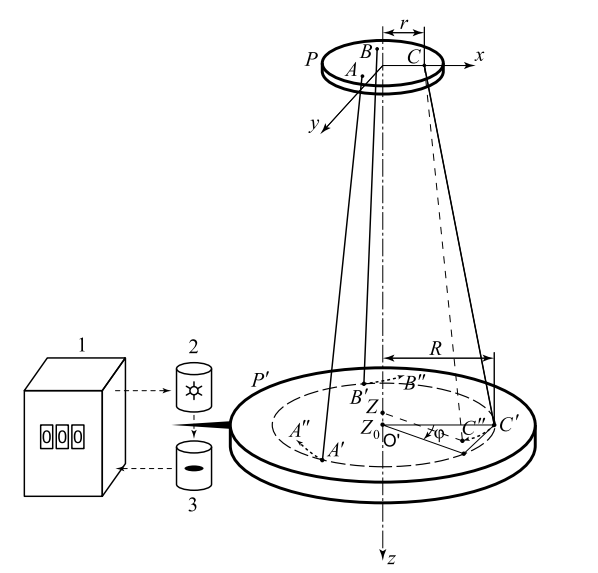
\includegraphics[width=0.95\linewidth]{ustan.png}
		\caption{Трифилярный подвес}
		\label{ust}
	\end{wrapfigure}
	
	Для наших целей удобно использовать устройство, показанное на Рис. \ref{ust} и называемое трифилярным подвесом. Оно состоит из укрепленной на некоторой высоте неподвижной платформы $P$ и подвешенной к ней на трех симметрично расположеных нитях $AA'$, $BB'$ и $CC'$, вращающейся платформы $P'$. 
	
	Чтобы не вызывать дополнительных раскачиваний, лучше поворачивать верхнюю платформу, укрепленную на неподвижной оси. После поворота верхняя платформа остается неподвижной в течение всего процесса колебний. После того, как нижняя платформа $P'$ оказывается повернутой на угол $\varphi$ относительно верхней платформы $P$, вощникает момент сил, стремящийся вернуть нижнюю платформу в положение равновесия, при котором относительный поворот платформ отсутствует. В результате платформа совершает крутильные колебания.
	
	\section{Теоретические сведения}
	
	\par Инерционность при вращении тела относительно оси определяется моментом инерции тела относительно этой оси. Момент инерции твердого тела относительно неподвижной оси вращения вычисляется по формуле:
	
	\begin{equation}
		I = \int r^2 dm
	\end{equation}
	
	Здесь $r$ -- расстояние элемента массы тела $dm$ от оси вращения. Интегрирование проводится по всей массе тела $m$.
	
	Если пренебречь потерями энергии на трение о воздух и крепление нитей, то уравнение сохранения энергии при коебаниях можно записать следующим образом:
	
	\begin{equation}\label{moment}
		\frac{I \dot{\varphi^2}}{2} + mg(z_0-z) = E
	\end{equation}
	
	Здесь $I$ -- момент инерции платформы вместе с исследуемым телом, $m$ -- масса платформы с телом, $\varphi$ -- угол поворота платформы от положения равновесия системы, $z_0$ -- координата по вертикали центра нижней платформы $O'$  при равновесии ($\varphi = 0$), $z$ -- координата той же точки при некотором угле поворота $\varphi$. Превый член в левой части уравнения -- кинетическач энергия вращения, второй член -- потенциальная энергия в поле тяжести, $E$ -- полная энергия системы (платформы с телом).
	
	Воспользуемся системой координат $x, y, z$, связанной с верхней платформой, как показано на Рис. \ref{risunok}. Координаты верхнего конца одной из нитей подвеса точки $C$ в этой системе -- $(r, 0, 0)$. Нижний конец данной нити $C'$, находящийся на нижней платформе, при равновесии имеет координаты $(R, 0, z_0)$, а при повороте платформы на угол $\varphi$ эта точка переходит в $C''$ с координатами $(Rcos\varphi, Rsin\varphi, z)$. расстояние между точками $C$ и $C''$ равно длине нити, поэтому, после некоторых преобразований, получаем: 
	
	\begin{center}
			$ (R\cos\phi - r)^2 + R^2\sin^2\phi + z^2 = L^2 $
			
			$ z^2 = L^2 - R^2 - r^2 + 2Rr\cos\phi \approx z^2_{0} - 2Rr(1 - \cos\phi) \approx z^2_{0} - Rr\phi^2 $
			
			$ z = \sqrt{z^2_{0} - Rr\phi^2} \approx z_{0} - \frac{Rr\phi^2}{2z_{0}} $
	\end{center}
	Подставляя $z$ в уравнение \eqref{moment}, получаем:
	\begin{equation}
		\frac{1}{2}I\dot{\varphi^2} + mg \frac{Rr}{2z_0}\varphi^2 = E
	\end{equation}
	Дифференцируя по времени и сокращая на $\dot\varphi$, находим уравнение крутильных колебаний системы:
	\begin{equation}
		I\ddot\varphi^2 + mg\frac{Rr}{2z_0}\varphi^2 = 0
	\end{equation}
	Производная по времени от $E$ равна нулю, так как потерями на трение, как уже было сказано выше, пренебрегаем.
	Решение этого уравнения имеет вид:
	
	\begin{equation}
		\varphi = \varphi_0 sin \left(\sqrt{\frac{mgRr}{Iz_0}}t + \theta\right)
	\end{equation}
	Здесь амплитуда $\varphi_0$ и фаза $\theta$ колебаний определяются начальными условиями. Период кртуильных полебаний нашей системы равен:
	
	\begin{equation}
		T = 2\pi \sqrt{\frac{Iz_0}{mgRr}}
	\end{equation}
	
	Из формулы для периода получаем:
	
	\begin{equation}\label{momin}
		I = \frac{mgRrT^2}{4 \pi^2z_0} = kmT^2
	\end{equation}
	\noindent где $k = \frac{gRr}{4\pi^2z_0}$ -- величина, постоянная для данной установки.
	
	\section{Задание}
	\subsection{Проверка установки}
	
	При выводе формул мы предполагали, что потери энергии, связанные с трением, малы, то есть мало затухание колебаний. Это значит, что теоретические вычисления будут верны, если выполняется условие:
	
	\begin{equation}
		\tau \gg T
	\end{equation}
	
	Проверим данное условие. При отклонении на угол $\alpha \approx 30^\circ$ время, закоторое амплитуда уменьшится в 2 раза, $\tau \approx 240\text{ с}$, а $T \approx 3\text{ с}$. Соотношение выполняется -- установка пригодна для проведение эксперимента.
	
	\subsection{Параметры установки и коэффицент $k$}
	
	Работа выполнялась на установке №7, ее параметры указаны в Таблице \eqref{param}
	\begin{table}[!ht]
		\begin{center}
		\begin{tabular}{|l|l|l|l|l|l|l|l|}
			\hline
			$Z_0$, см & $\sigma_{Z_0}$, см & R, мм  & $\sigma_R$, мм & r, мм & $\sigma_r$, мм  & m, г & $\sigma_m$, г  \\ \hline
			206 & 1 & 115,4 & 0,5 & 30,5 & 0,3 & 993,5 & 0,5 \\ \hline
		\end{tabular}
		\caption{Парметры установки}
		\label{param}
		\end{center}
	\end{table}
	
	\noindent где $\sigma_m$, $\sigma_R$, $\sigma_r$, $\sigma_L$, $\sigma_{z_0}$ -- погрешности соответсвующих величин.
	
	\bigskip
	
	По полученным данным вычислим постоянную для конструкции №3:
	
	\begin{equation}
		k = \frac{gRr}{4\pi^2z_0} \approx 4,24395\cdot 10^{-4} \frac{\text{м}^2}{\text{с}^2}
	\end{equation}
	
	Погрешность же $k$ будет равна:
	
	\begin{equation}
		\sigma_k = k \cdot \sqrt{\left( \frac{\sigma_R}{R}\right)^2 + \left( \frac{\sigma_r}{r}\right)^2 + \left( \frac{\sigma_{z_0}}{z_0}\right)^2} \approx 0,05 \cdot 10^{-4} \frac{\text{м}^2}{\text{с}^2}
	\end{equation}
	
	\subsection{Момент инерции платформы}
	
	Определить момент инерции платформы можно по формуле \eqref{momin}. Для этого нам необходимо определить период колебаний ненагруженной платформы. Измеряем преиод, получаем:
	
	\begin{table}[!ht]
		\begin{center}
			\begin{tabular}{|l|l|l|l|l|}
				\hline
				 T, c & N & Tср, с & $A_0$ & $A_k$ \\ \hline
			     134,452 & 30 & 4,482 & 35 & 25 \\ \hline
			\end{tabular}
		\end{center}
	\end{table}
	
	Тогда, средний период колебания платформы будет: $T_\text{ср} \approx 4,482\text{, с}$
	
	Давайте здесь же и определим погрешность времени: 
	
    $$\sigma_T^{\text{сист}} = 0,001\text{, с}\;\;\;\;\sigma_N = 0,5$$
	$$\sigma_{T_\text{ср}} = T_\text{ср}\sqrt{\varepsilon_T^{2} + \varepsilon_{N}^{2}} =\approx 0,075\text{, с}$$

	Значит $T_\text{ср} = \left(4,482 \pm 0,075\right)\text{с}$. Теперь мы можем определить момент инерции платформы:
	
	\begin{equation}
		I_\text{пл} = kmT^2 \approx 8,469  \text{,  кг $\cdot$ $\text{м}^2$ $\cdot 10^{-3}$}  
	\end{equation}
	
	Найдем погрешность найденного нами момента инерции платформы:
	
	\begin{equation}
		\varepsilon_I = \sqrt{ \left(\frac{\sigma_k}{k}\right)^2 +\left(\frac{\sigma_m}{m}\right)^2 + \left(2\frac{\sigma_T}{T}\right)^2} \approx 0,035
	\end{equation}
	\begin{equation}
		\sigma_{I_\text{пл}} = \varepsilon_I \cdot I_\text{пл} \approx 0,295 \text{,  кг $\cdot$ $\text{м}^2$ $\cdot 10^{-3}$}
	\end{equation}
	Получаем, что с помощью данной конструкции мы можем определять момент инерции тела с погрешностью 3,5\%, и $I_\text{пл} = \left(8,469 \pm 0,295\right) \text{,  кг $\cdot$ $\text{м}^2$ $\cdot 10^{-3}$}$
	
	\subsection{Определение моментов инерции различных тел. Аддитивность моментов инерции}
	
	Измерим периоды колебаний платформы с различными телами таким же образом, как и для ненагруженной платформы. Данные полученный в результате измерений представлены в таблице ниже:
	
	\begin{table}[!ht]
		\begin{center}
		\begin{tabular}{|l|l|l|l|l|l|l|l|l|}
			\hline
			1 & стержень & m, г & $\sigma_m$, г & T, c & N & Tср, с & $A_0$ & $A_k$ \\ \hline
			I, кг*м\^2 & 0,01115 & 1039,40 & 0,05 & 115,030 & 32 & 3,595 & 25 & 20 \\ \hline
			2 & полуцилиндры & m, г & $\sigma_m$, г & T, c & N & Tср, с & $A_0$ & $A_k$ \\ \hline
			I, кг*м\^2 & 0,01003 & 1442,20 & 0,05 & 93,448 & 30 & 3,115 & 25 & 20 \\ \hline
			3 & полый циллиндр & m, г & $\sigma_m$, г & T, c & N & Tср, с & $A_0$ & $A_k$\\ \hline
			I, кг*м\^2 & 0,01348 & 777,20 & 0,05 & 127,043 & 30 & 4,235 & 30 & 25 \\ \hline
			4 & диск & m, г & $\sigma_m$, г & T, c & N & Tср, с & $A_0$ & $A_k$ \\ \hline
			I, кг*м\^2 & 0,01068 & 584,40 & 0,05 & 119,797 & 30 & 3,993 & 35 & 30 \\ \hline
		\end{tabular}
		\caption{Моменты инерции платформы с различными телами}
		\label{momtel}
		\end{center}
	\end{table}
	Для подтверждения аддитивности необходимо показать,что выполняются условия:
	\begin{equation} \label{plc}
		I_\text{пл+д} = I_\text{пл} + I_\text{д}
	\end{equation}
	\begin{equation}\label{plk}
		I_\text{пл+пол.ц.} = I_\text{пл} + I_\text{пол.ц.}
	\end{equation}
	\begin{equation}
		I_\text{пл+д+пол.ц.} = I_\text{пл} + I_\text{д} + I_\text{пол.ц.}
		\label{plck}
	\end{equation}
	\begin{equation}
		(3) + (4) + (5) \Rightarrow I_\text{пл+д+пол.ц.} = I_\text{д + пл} + I_\text{пол.ц. + пл} - I_\text{пл}
	\end{equation}
Подставим в правую часть последней формулы данные из таблицы \eqref{momtel} и сравним с экспериментально полученной левой частью:   
\begin{table}[!h]
	\begin{center}
	\begin{tabular}{|c|c|c|c|c|c|c|c|c|}
		\hline
		$I_\text{д + пл} + I_\text{пол.ц. + пл} - I_\text{пл}$ &  $I_\text{пл+д+пол.ц.}$ & m, г & dm, г & T, c & N & Tср, с & A0 & Ak \\ \hline
		 0,01569 & 0,01573 & 1361,60 & 0,05 & 158,793 & 40 & 3,969825 & 30 & 25 \\ \hline
	\end{tabular}
	\end{center}
\end{table}
	
	\noindent Из таблицы видно, что $I_\text{д + пл} + I_\text{пол.ц. + пл} - I_\text{пл}$ и  $I_\text{пл+д+пол.ц.}$ хорошо сходятся, то есть условие аддитивности выполняется.
	
	Из Таблицы \eqref{momtel} и формул \eqref{plc}, \eqref{plk} мы можем найти момент инерции полого цилиндра, диска, стержня и полуцилиндров:
	 $$I_\text{пол.ц.} = I_\text{пл+пол.ц.} - I_\text{пл} = \left(5,011 \pm 0,768\right) \text{,  кг $\cdot$ $\text{м}^2$ $\cdot 10^{-3}$}\text{ ,}$$
	 $$I_\text{д} = I_\text{пл+д} - I_\text{пл} = \left(2,211 \pm 0,670\right) \text{,  кг $\cdot$ $\text{м}^2$ $\cdot 10^{-3}$}\text{ ,}$$
	 $$I_\text{ст} = I_\text{пл+ст} - I_\text{пл} = \left(2,681 \pm 0,687\right) \text{,  кг $\cdot$ $\text{м}^2$ $\cdot 10^{-3}$}\text{ и}$$
	 $$I_\text{полуц} = I_\text{пл+полуц} - I_\text{пл} = \left(1,561 \pm 0,647\right) \text{,  кг $\cdot$ $\text{м}^2$ $\cdot 10^{-3}$}.$$
	
	Теперь сравним полученные нами моменты инерциии для тел, и их теоретические значения. Для цилиндра (двух полуцилиндров) момент инерции вычисляется так же как и для диска: $I_\text{полуц} = \frac{m_\text{ц}R_\text{ц}^2}{2} = I_\text{д}$. 
	Для стержня: $I_\text{ст} = \frac{ml^2}{12}$. 
	\\Для полого цилиндра же: $I_\text{пол.ц.} = \frac{m_\text{пол.ц.}(R_\text{внеш}^2 + R_\text{внутр}^2)}{2}$. 
	\\ В следующей таблице представленный геометричиские характеристики всех тел и их моменты инерций рассчитанные по формулам сверху:
	\begin{table}[!ht]
		\centering
		\begin{tabular}{|l|l|l|l|l|l|l|l|}
			\hline
			1 & cтержень & l, см & $\sigma_l$, см & a, см & $\sigma_a$, см & ~ & ~  \\ \hline
			I, кг*м\^2 & 0,00250 & 17,0 & 0,1 & 2,710 & 0,005 & ~ & ~  \\ \hline
			2 & полуцилиндры & R, см & $\sigma_R$, см & a, см & $\sigma_a$, см & ~ & ~  \\ \hline
			I, кг*м\^2 & 0,00147 & 5 & 0,005 & 2,7 & 0,005 & ~ & ~ \\ \hline
			3 & полый циллиндр & D, см & $\sigma_D$, см & a, см & $\sigma_d$, см & H, см & $\sigma_H$, см  \\ \hline
			I, кг*м\^2 & 0,00478 & 15,9 & 0,01 & 0,435 & 0,005 & 5,650 & 0,005  \\ \hline
			4 & диск & D, см & $\sigma_D$, см & a, см & $\sigma_a$, см & h, см & $\sigma_h$  \\ \hline
			I, кг*м\^2 & 0,00212 & 17,03 & 0,01 & 0,350 & 0,005 & 2,6 & 0,005  \\ \hline
		\end{tabular}
	\end{table}
	
	
	\subsection{Зависимость момента инерции системы тел от их расположения. График зависимости $I(h^2)$}
	\begin{wrapfigure}[10]{r}{0.25\textwidth}
		\vspace{-3em}
		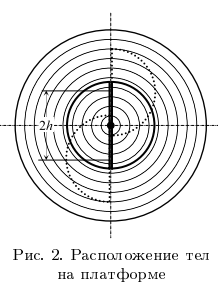
\includegraphics[width=0.25\textwidth]{rasp}
	\end{wrapfigure}

	Определим зависимость момента инерции системы двух тел от их взаимного расположения. Для этого располагая грузы, как показано на рис.2, получим зависимость от расстояния. Затем Используя формулу \ref{momin}, определим зависимость $I(h^2)$.

	Полученные результаты измерений занесем в таблицу снизу соответсвенно. Основывыаясь на результатах таблицы \eqref{tab:moment}, построим график зависимости $ I(h^{2}) $ (Рис. \ref{ris:grafik}).
	\bigskip\bigskip\bigskip\bigskip\bigskip
	
\begin{table}[!ht]
	\centering
	\vspace{-3em}
	\begin{tabular}{|l|l|l|l|l|l|l|l|l|}
		\hline
		парал & сдвиг & T, c & N & Tср, с & h, см & dh, см & $h^2$, $\text{м}^2$ & I, кг*$\text{м}^2$ \\ \hline
		1 & 2h = 4 деления & 95,043 & 30 & 3,168 & 2 & 0,008 & 0,0004 & 0,01038 \\ \hline
		2 & 2h = 8 делений & 112,405 & 35 & 3,212 & 4 & 0,016 & 0,0016 & 0,01066 \\ \hline
		3 & 2h = 12 делений & 99,983 & 30 & 3,333 & 6 & 0,024 & 0,0036 & 0,01148 \\ \hline
		4 & 2h = 16 делений & 123,285 & 35 & 3,522 & 8 & 0,032 & 0,0064 & 0,01283 \\ \hline
		5 & 2h = 20 делений & 111,021 & 30 & 3,701 & 10 & 0,04 & 0,01 & 0,01416 \\ \hline
		6 & 2h = 24 деления & 140,084 & 36 & 3,891 & 12 & 0,048 & 0,0144 & 0,01565 \\ \hline
		7 & 2h = 28 делений & 123,652 & 30 & 4,122 & 14 & 0,056 & 0,0196 & 0,01756 \\ \hline
		перп & 0 делений & 93,448 & 30 & 3,115 & 0 & 0 & 9,703 & 0,01003 \\ \hline
		1 & 2h = 4 деления & 97,379 & 30 & 3,246 & 2 & 0,008 & 0,0004 & 0,01089 \\ \hline
		2 & 2h = 8 делений & 101,884 & 30 & 3,396 & 4 & 0,016 & 0,0016 & 0,01192 \\ \hline
		3 & 2h = 12 делений & 107,324 & 30 & 3,577 & 6 & 0,024 & 0,0036 & 0,01323 \\ \hline
		4 & 2h = 16 делений & 112,717 & 30 & 3,757 & 8 & 0,032 & 0,0064 & 0,01459 \\ \hline
		5 & 2h = 20 делений & 121,002 & 30 & 4,033 & 10 & 0,04 & 0,01 & 0,01682 \\ \hline
		6 & 2h = 24 деления & 112,58 & 26 & 4,330 & 12 & 0,048 & 0,0144 & 0,01938 \\ \hline
	\end{tabular}
	\caption{Зависимость момента инерции системы от расстояния}
	\label{tab:moment}
\end{table}
	
	\begin{figure}[!h]
		\begin{center}
			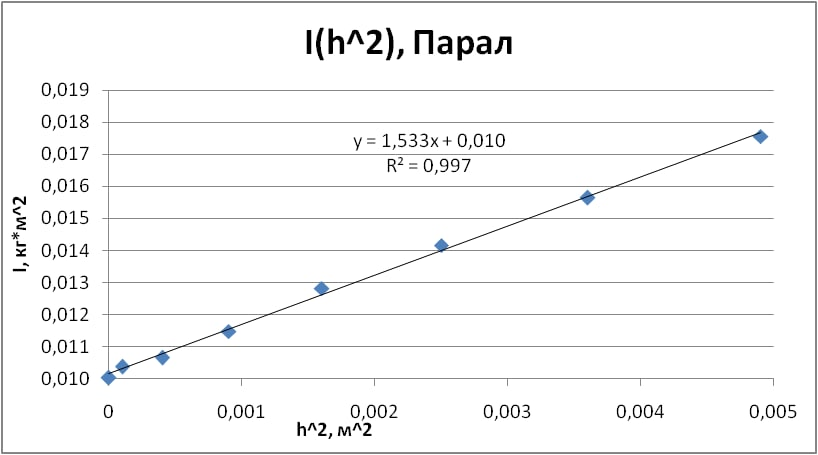
\includegraphics[width=1\textwidth]{graph_1}
			%\includegraphics[width=0.45\textwidth]{graph_2}
			\caption{График зависимости $ I(h^2) $}
			\label{ris:grafik}
		\end{center}
	\end{figure}

	По левому графику понятно, что $I = kh^2 + b$. 
	Тогда $b$ -- момент инерции платформы + полуцилиндров($I_\text{пл + цил}$), т.е. $b = I_\text{пл} + \frac{m_\text{цил} R^2}{2}$. 
	\newpage
	По теореме Гюйгенса-Штейнера должно выполняться:
	$$(I - I_\text{пл} =) I'_\text{цил} = m_\text{цил} h^2 + I_\text{цил} \Leftrightarrow I = m_\text{цил} h^2 + I_\text{цил} + I_\text{пл} $$
,т.е. для подтверждения формулы Гюйгенса-Штейнера необходимо показать, что:
$$k = m_\text{цил} \text{ и } b = I_\text{цил} + I_\text{пл}$$
 Для вычисления коэффициентов $ k $ и $ b $ (левого графика) воспользуемся методом наименьших квадратов:
		
	\begin{equation}
		k=\frac{\langle xy\rangle-\langle x\rangle \langle y\rangle}{\langle x^2\rangle - \langle x\rangle^2}\approx 1,534\text{, } \frac{\text{кг}\cdot\text{м}^2}{\text{м}^2},
	\end{equation}
	
	\begin{equation}
		b=\langle y \rangle -k\langle x \rangle\approx 0,01016\text{,  кг $\cdot$ $\text{м}^2$},
	\end{equation}
	где $ x=h^2 $, $ y=I $.
	
	Случайные погрешности вычисления $ k $ и $ b $ можно найти по следующим формулам:
	
	\begin{equation}
		\sigma_k^\text{случ}=\frac{1}{\sqrt{N}}\sqrt{\frac{\langle y^2 \rangle - \langle y \rangle^2}{\langle x^2 \rangle - \langle x \rangle^2} - k^2  } \approx 0,026
		 \text{, } \frac{\text{кг}\cdot\text{м}^2}{\text{м}^2},
	\end{equation}
	
	\begin{equation}
		\sigma_b^\text{случ}= \sigma_k^\text{случ} \sqrt{\langle x^2 \rangle - \langle x \rangle^2} \approx 0,00004
		\text{,  кг $\cdot$ $\text{м}^2$}.
	\end{equation}
	
	Систематическая погрешность вычисления коэффициентов определяется следующим соотношением:
	
	\begin{equation}
		\sigma^\text{сист}_b = b\sqrt{\left( \varepsilon_{I} \right)^2 + \left( \varepsilon_{h^2} \right)^2 } \approx b \cdot \varepsilon_I \approx 0,00036 \text{,  кг $\cdot$ $\text{м}^2$}.
	\end{equation}
	
	Тогда полную погрешность вычисления коэффициентов подсчитываем по следующей формуле:
	
	\begin{equation}
		\sigma_b = \sqrt{\left( \sigma_b^\text{случ} \right)^2 + \left( \sigma_b^\text{сист} \right)^2 } \approx 0,00036 \text{,  кг $\cdot$ $\text{м}^2$}.
	\end{equation}
	Таким образом $k = (1,534 \pm 0,026)\text{кг}$ неплохо ($3,5\sigma_k$) совпадает с $m_\text{цил} = 1442 \text{ г}$ и $b = (10,16 \pm 0,36)\text{ кг} \cdot \text{м}^2$ хорошо ($\sigma_b$) совпадает с $I_\text{пл + цил} = 10,03\text{ кг} \cdot \text{м}^2 $
	Значит теорема Гюйгенса-Штейнера выполняется.
	\section{Вывод}
	
	С помощью трифилярного подвеса можно определять момент инерции тел, момент инерции которых больше момента инерции самой платформы, с достаточно большой точностью. В проведенном эксперименте моменты инерции тел были определены с $\varepsilon_I$ от $15\%$ до $40\%$. Такая погрешность обусловлена несовершенством датчика фиксирующего колебания и человеческим фактором.
	
	Мы экспериментально доказали аддитивность моментов инерции с помощью различных тел.
	
	Полученная зависимость $I(h^2)$ аппроксимируется линейой зависимостью, что подвтерждает формулу Гюйгенса-Штейнера ($I = I_c + Mh^2$, где $I$ -- момент инерции тела, $I_c$ --момент инерции тела относительно центра, $M$ -- масса тела, а $h$ -- расстояние между двумя осями, в нашем случае -- между осью вращения и половинками диска).
	
\end{document}